\documentclass[DIV=calc, paper=a4, fontsize=11pt, twocolumn]{scrartcl}
\usepackage{microMathematics-ru}
\usepackage[russian]{babel}
\usepackage{hyphsubst}

% Begin document
\begin{document}
\maketitle
\thispagestyle{fancy} % Enabling the custom headers/footers for the first page

\begin{bf}
% This is the first part of the file about_micromath_ru.tex
microMathematics Plus - это
математический калькулятор для
Android, основанный на подготовке
интерактивных документов с
вычислениями и визуальным
сопровождением.

Он базируется на мощном
пальце-ориентированном редакторе
формул, который позволяет
пользователям создавать,
редактировать и вычислять формулы
в стандартном математическом виде.

microMathematics Plus поддерживает
вычисления на уровне начальных
курсов высших учебных заведений,
но имеет следующие ограничения:
приложение не поддерживает
специальные функции, векторы,
матрицы и многие другие аспекты
высшей математики.
\end{bf}

\section{Описание программы}
% This is auto-generated file: do not edit!
% Exported from microMathematics, version 1.23


Данное приложение является мощным
математическим калькулятором,
который основан на работе с
интерактивными документами.
Приложение содержит один рабочий
лист, его можно изменять,
вычислять, сохранять на SD карту,
а также экспортировать в документ
LaTeX или изображение.

Рабочий лист - это полноценный
документ с текстом, формулами и
графиками. Математические объекты
в нём можно редактировать и
вычислять в том виде, как они
выглядят на экране.

Доступны следующие типы объектов:
формула, текстовый результат,
график функции, текстовое поле и
изображение. В данном разделе
даётся краткое описание того, как
работать с этими объектами.

\subsection{Редактирование}

Большинство объектов содержат поля,
которые можно редактировать. Для
редактирования используйте кнопки
на нижней панели инструментов, с
их помощью можно вводить
математические символы в поля
объекта.

Символы с этой панели также можно
ввести и с клавиатуры. Чтобы
узнать символ, соответствующий
кнопке, посмотрите подсказку,
всплывающую при долгом нажатии на
кнопку.

При долгом нажатии на часть
формулы активируется контекстное
меню. В нём выбранную часть можно
удалить, скопировать в буфер
обмена, заменить выражением из
буфера, а также вставить после неё
оператор или функцию, используя
панель инструментов или
клавиатуру.

Для отмены неудачного действия
можно использовать команду
главного меню ''Отменить ввод'':
\begin{center}\begin{tabular}{c} 
\includegraphics[width=0.45\textwidth]{graphics/how_to_use_fig1.png} \end{tabular}\end{center}

\subsection{Формула}

Формула определяет константу,
интервал, или функцию. Для
добавления формулы используйте
кнопку ''Вставить'' на верхней
панели инструментов
\begin{center}\begin{tabular}{c} 
\includegraphics[width=0.45\textwidth]{graphics/how_to_use_fig2.png} \end{tabular}\end{center}

или кнопку ''Вставить формулу'' на
нижней панели:
\begin{center}\begin{tabular}{c} 
\includegraphics[width=0.45\textwidth]{graphics/how_to_use_fig3.png} \end{tabular}\end{center}

После этого появится объект с двумя
пустыми полями, обязательными для
заполнения:
\begin{center}\begin{tabular}{c}
  ${\Box} := {\Box}$
\end{tabular}\end{center}

В левом поле объекта вводится имя
формулы. Имя должно содержать
только буквы или цифры и может
быть использовано далее в других
формулах.

Из верхней панели инструментов
можно вызвать окно ''Свойства
документа'': 
\begin{center}\begin{tabular}{c} 
\includegraphics[width=0.45\textwidth]{graphics/how_to_use_fig4.png} \end{tabular}\end{center}

В зависимости от параметра
''Разрешить переопределение
формул'', доступного в этом
диалоге, возможны два режима:

а) Если переопределение формул не
разрешено, то имя формулы должно
быть уникальным для всего
документа и эту формулу можно
использовать как до, так и после
её определения.

б) Если переопределение разрешено,
то можно определить несколько
формул с одним и тем же именем, но
при ссылке на неё будет
использован самый последний
вариант, определённый перед
вызывающим объектом.

\subsubsection{Формула - константа}

Если имя формулы не содержит
аргумента в круглых скобках, то
такая формула определяет константу
или интервал. Константа задаёт
какое-либо одно число, которое
определяется правой частью:
\begin{center}\begin{tabular}{ccc}
  $N := 200$ &
  $Sq2 := \sqrt{100} $ &
  $Pi2 := \frac{{\pi}}{2}$ \cr
\end{tabular}\end{center}

Последний пример демонстрирует
использование встроенной константы
пи. Пока доступны следующие
встроенные константы:
\begin{center}\begin{tabular}{ccc}
  ${\pi} = 3.14159$ &
  $pi = 3.14159$ &
  $e = 2.71828$ \cr
\end{tabular}\end{center}

В правой части можно также
использовать любую константу,
определённую ранее:
\begin{center}\begin{tabular}{c}
  $NPi2 := N \cdot Pi2$
\end{tabular}\end{center}

Для обозначения комплексной
константы используйте символ
мнимой единицы i:
\begin{center}\begin{tabular}{c}
  $z := 5 + 3i$
\end{tabular}\end{center}

\subsubsection{Формула - интервал}

Формула интервального типа задаёт
переменную, которая изменяется в
заданном интервале с определённым
шагом. Эта переменная служит для
задания аргументов функции при
построении графиков или выводе
таблиц значений.

Для того чтобы задать интервал, в
левом поле введите его имя, а в
пустом правом поле введите символ
'':'' или нажмите на кнопку
''Интервал'' на нижней панели
инструментов:
\begin{center}\begin{tabular}{c} 
\includegraphics[width=0.45\textwidth]{graphics/how_to_use_fig5.png} \end{tabular}\end{center}

Первый элемент с индексом 0
определяет начальное значение,
второй элемент с индексом 1
определяет следующие значение, а
третий элемент задаёт конечное
значение интервала:
\begin{center}\begin{tabular}{c}
  $x := \left[ 0,\, 0.1 \,..\, 10 \right]$
\end{tabular}\end{center}

Обращаться к элементам интервала
нужно по индексу:
\begin{center}\begin{tabular}{ccc}
  $x \left( 0\right)  = 0.0$ &
  $x \left( 1\right)  = 0.1$ &
  $x \left( 100\right)  = 10.0$ \cr
\end{tabular}\end{center}

Шаг определятся как разница двух
соседних элементов:
\begin{center}\begin{tabular}{c}
  $x \left( 2\right)  - x \left( 1\right)  = 0.1$
\end{tabular}\end{center}

К примеру, задать интервал с
нулевым начальным значением и
содержащий N точек, равномерно
распределённых с шагом ''dy'', можно
таким образом:
\begin{center}\begin{tabular}{cc}
  $dy := 0.05$ &
  $y := \left[ 0,\, dy \,..\, dy \cdot N \right]$ \cr
\end{tabular}\end{center}

\subsubsection{Формула - функция}

Функция определяет зависимость
между одним или несколькими
аргументами и областью значений,
где каждое значение вещественного
или комплексного аргумента или
комбинации аргументов даёт нам
только одно итоговое значение
функции.

Имя функции и её аргументы (в
круглых скобках через запятую)
указываются в левом поле.
Переменную, обозначающую аргумент,
не обязательно определять ранее -
можно использовать любое
обозначение, содержащее буквы и
цифры:
\begin{center}\begin{tabular}{c}
  $f(t) := sin \left( t\right)  \cdot cos \left( t\right)  / 2$
\end{tabular}\end{center}
\begin{center}\begin{tabular}{c}
  $w(z) := {e}^{2i \cdot {\pi} \cdot z}$
\end{tabular}\end{center}
\begin{center}\begin{tabular}{c}
  $H(x,y) := \sqrt{{x}^{2} + {y}^{2}} $
\end{tabular}\end{center}
\begin{center}\begin{tabular}{c}
  $g(x,y) := \frac{sin \left( H \left( x,\, y\right) \right) }{H \left( x,\, y / 2\right)  + 1}$
\end{tabular}\end{center}

Правая часть такого объекта
содержит математическое выражение
для вычисления функции. Если
правая часть не содержит ни одного
аргумента из левой части, то такая
функция будет интерпретироваться
как константа.

В правой части можно использовать
другие функции, как встроенные,
так и определённые ранее. Для
этого введите имя функции, затем
символ ''('', а затем её аргумент.
Аргумент также может быть формулой
с любыми операторами и функциями.

Список всех встроенных функций
содержится в документе
''functions\_overview.mmt'', который
находится в ресурсах приложения.

\subsection{Текстовый результат}

Этот элемент предназначен для
просмотра результатов вычислений в
текстовом виде: как одно число или
как массив чисел. Для добавления
этого элемента используйте кнопку
''Вставить'' на верхней панели
инструментов или кнопку ''Вставить
текстовый результат'' на нижней
панели:
\begin{center}\begin{tabular}{c} 
\includegraphics[width=0.45\textwidth]{graphics/how_to_use_fig6.png} \end{tabular}\end{center}

После этого появится объект с двумя
пустыми полями, где левое поле
необходимо заполнить:
\begin{center}\begin{tabular}{c}
  ${\Box} = {\Box}$
\end{tabular}\end{center}

Левое поле может содержать любое
математическое выражение, а в
правом будет показан результат
после нажатия плавающей кнопки
''Вычислить''.

В левом поле можно использовать
любые константы и функции, как
встроенные, как и определённые
ранее:
\begin{center}\begin{tabular}{c}
  ${e}^{{\pi}} \cdot f \left( NPi2\right)  = 2.27286E-14$
\end{tabular}\end{center}

Если левая часть не зависит от
переменных интервального типа, то
результатом вычислений будет одно
вещественное или комплексное
число:
\begin{center}\begin{tabular}{c}
  $y \left( N - 1\right)  - y \left( 0\right)  = 9.95$
\end{tabular}\end{center}
\begin{center}\begin{tabular}{ccc}
  $\Re\left( z \right)  = 5.0$ &
  $\Im\left( z \right)  = 3.0$ &
  $ \left| z \right|  = 5.83095$ \cr
\end{tabular}\end{center}
\begin{center}\begin{tabular}{c}
  $\sqrt{sin \left( \frac{3}{2} \cdot {\pi}\right) }  = 0.0+1.0i$
\end{tabular}\end{center}

Если слева используется интервал,
то результат будет массивом чисел,
соответствующих интервалу. Ввиду
ограниченности дисплея, будут
показаны только несколько первых и
последнее число из этого массива:
\begin{center}\begin{tabular}{ccc}
  $x = \begin{bmatrix}0.0\\0.1\\0.2\\0.3\\0.4\\0.5\\\dots\\10.0\\\end{bmatrix}$ &
  $y = \begin{bmatrix}0.0\\0.05\\0.1\\0.15\\0.2\\0.25\\\dots\\10.0\\\end{bmatrix}$ &
  $2 \cdot y = \begin{bmatrix}0.0\\0.1\\0.2\\0.3\\0.4\\0.5\\\dots\\20.0\\\end{bmatrix}$ \cr
\end{tabular}\end{center}

Количество показанных элементов, а
также режим вычисления и показа
поля результата можно изменить в
настройках формулы. Для вызова
окна настроек необходимо выделить
всю формулу целиком, после чего
появится плавающая кнопка
''Настройки объекта'', по нажатии на
которую и откроется окно настроек:
\begin{center}\begin{tabular}{c} 
\includegraphics[width=0.45\textwidth]{graphics/how_to_use_fig7.png} \end{tabular}\end{center}

Также появится вторая плавающая
кнопка - ''Подробности''. При
нажатии на неё откроется окно, где
будут показаны все элементы
массива.

Обратите внимание, что данная
версия программы не поддерживает
использование двух и более
переменных интервального типа в
объекте текстового результата.

\subsection{График функции}

Данный элемент предназначен для
отображения графиков функций одной
переменной. Для добавления
используйте кнопку ''Вставить'' на
верхней панели инструментов или
кнопку ''Вставить график функции''
на нижней панели:
\begin{center}\begin{tabular}{c} 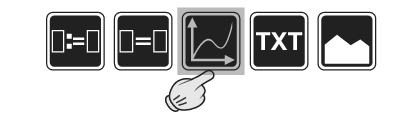
\includegraphics[width=0.45\textwidth]{graphics/how_to_use_fig8.png} \end{tabular}\end{center}

Появится поле графика с шестью
пустыми полями. Функция, для
которой строится график, задаётся
в левом среднем поле, а аргумент
функции указывается в нижнем
среднем поле:
\begin{center}\begin{tabular}{c} 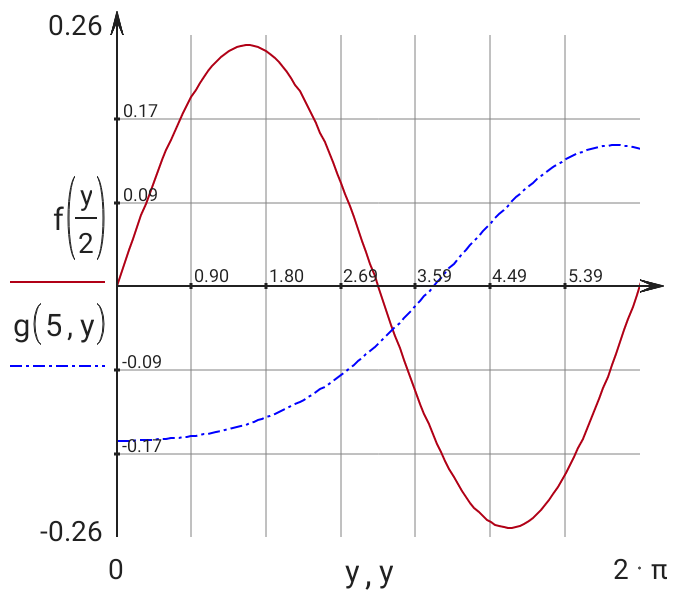
\includegraphics[width=0.45\textwidth]{graphics/how_to_use_fig9.png} \end{tabular}\end{center}

Для более подробного ознакомления с
графиком функции см. примеры
''График функции'' и ''Полярный
график'' из навигатора приложения.

\subsection{Текстовое поле}

Этот элемент служит для ввода
простого текста. Добавить
текстовое поле можно кнопкой
''Вставить'' на верхней панели
инструментов или кнопкой ''Вставить
текстовое поле'' на нижней панели:
\begin{center}\begin{tabular}{c} 
\includegraphics[width=0.45\textwidth]{graphics/how_to_use_fig10.png} \end{tabular}\end{center}

Если при помощи контекстного меню
''Выбрать всё'' выделить весь текст
фрагмента, то появится плавающая
кнопка ''Настройки объекта''. 

При нажатии на эту кнопку
откроется окно настроек текста,
где можно изменить его стиль и
нумерацию. Например, заголовки
глав в данном документе имеют тип
''Глава'' со включенной
автоматической нумерацией.

\subsection{Изображение}

Если есть файл с изображением,
которое хотелось бы внедрить в
документ в виде иллюстрации, то
это также можно сделать. Для этого
нужно выбрать кнопку ''Вставить'' на
верхней панели инструментов или
кнопку ''Вставить изображение из
файла'' на нижней панели:
\begin{center}\begin{tabular}{c} 
\includegraphics[width=0.45\textwidth]{graphics/how_to_use_fig11.png} \end{tabular}\end{center}

После этого откроется окно
настройки изображения, где можно
выбрать нужный файл и задать
желаемые размеры.

Программа поддерживает файлы
следующих форматов: png, bmp, gif,
jpeg, svg.

Если в окне настроек установить
флаг ''Внедрить в документ'', то
изображение будет сохранено внутри
документа. Это увеличивает размер
файла документа, но позволяет его
использовать в дальнейшем, даже
если файл с изображением будет
удалён.

Если же флаг ''Внедрить в документ''
не установлен, то внутри документа
будет сохранён только путь к
файлу. В этом случае, файл с
изображением нужно всегда
копировать вместе с документом.

Свойства внедрённого изображения
можно изменить. Для этого долгим
нажатием на картинке дождитесь
появления плавающей кнопки
''Настройки объекта'', при нажатии
на которую появится окно со
свойствами этой картинки.

\section{Пример: график функции}
% This is auto-generated file: do not edit!
% Exported from microMathematics Plus, version 2.23.0


Данный пример демонстрирует
построение и возможности настройки
графиков функций. Построим графики
трёх следующих функций:
\begin{center}\begin{tabular}{c}
  $f(x) := 25 + 10 \cdot sin \left( \sqrt{ \left| x \right| } \right) $
\end{tabular}\end{center}
\begin{center}\begin{tabular}{c}
  $g(x) := \frac{2}{{e}^{ \left| x \right|  / 15}} \cdot f \left( x \cdot 50\right) $
\end{tabular}\end{center}
\begin{center}\begin{tabular}{c}
  $h(x) := min \left( f \left( x\right) ,\, g \left( x\right) \right) $
\end{tabular}\end{center}

Значение аргумента функции, которое
откладывается по оси x, будет
изменяться в интервале от x1 до x2
и содержать N точек:
\begin{center}\begin{tabular}{ccc}
  $N := 300$ &
  $x1 := -30$ &
  $x2 := 30$ \cr
\end{tabular}\end{center}
\begin{center}\begin{tabular}{c}
  $x := \left[ x1,\, x1 + \left( x2 - x1 \right) / N \,..\, x2 \right]$
\end{tabular}\end{center}

После того, как функции и их
аргументы определены, можно
добавить поле графика, используя
кнопку ''Вставить'' на верхней
панели действий или кнопку
''Вставить график функции'' на
нижней панели:
\begin{center}\begin{tabular}{c} 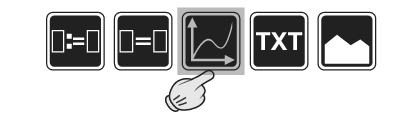
\includegraphics[width=0.45\textwidth]{graphics/function_plot_fig1.png} \end{tabular}\end{center}
\begin{center}\begin{tabular}{c} 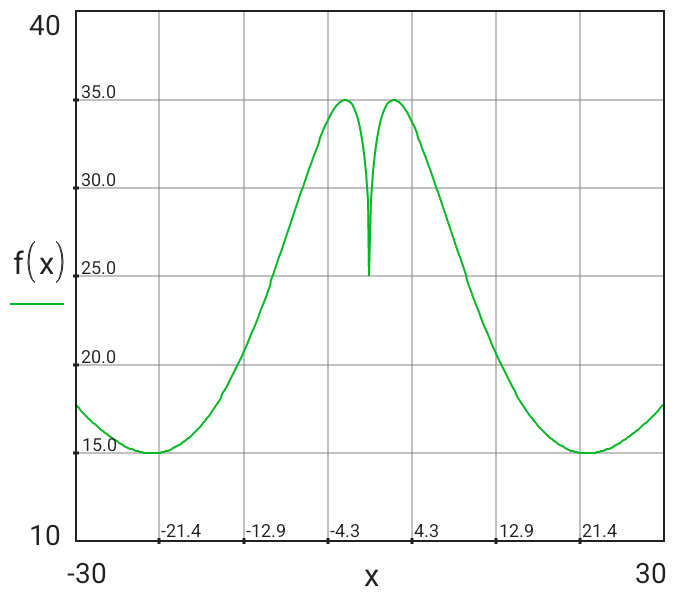
\includegraphics[width=0.45\textwidth]{graphics/function_plot_fig2.png} \end{tabular}\end{center}

Функция, для которой строится
график, задаётся в левом среднем
поле. В нём можно использовать
любые встроенные или введённые
ранее функции, а также выражение,
содержащее любые операции.

В нижнем среднем поле указывается
аргумент функции, для которого
строится график. Аргументом может
быть как переменная интервального
типа, так и любое выражение, явно
содержащее такую переменную.

Остальные четыре поля служат для
задания областей значений
аргумента и функции. Если эти поля
оставить пустыми, то программа
вычислит их автоматически. Однако,
эти автоматические значения можно
редактировать и изменять вручную.

Можно строить в одном поле графики
сразу нескольких функций. Для
добавления ещё одной функции
необходимо выделить (долгим
нажатием в левом среднем поле) ту
функцию, после которой нужно
добавить новую, и затем нажать
кнопку ''Вставить аргумент'' на
нижней панели инструментов:
\begin{center}\begin{tabular}{c} 
\includegraphics[width=0.45\textwidth]{graphics/function_plot_fig3.png} \end{tabular}\end{center}
\begin{center}\begin{tabular}{c} 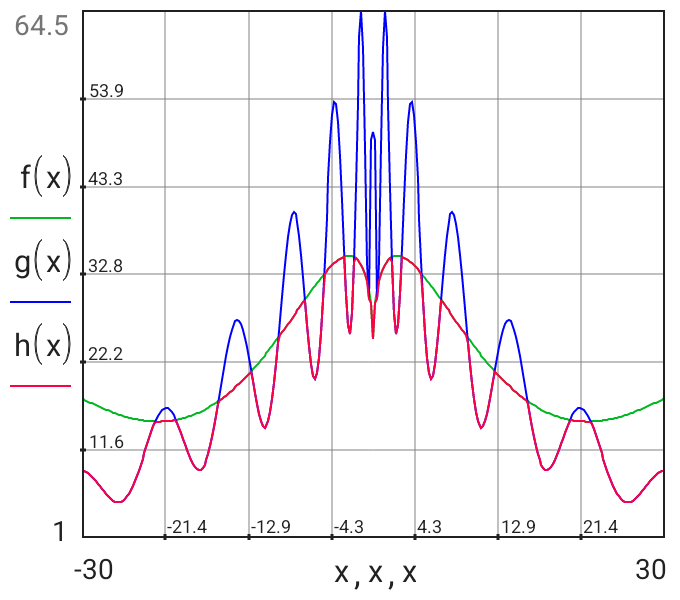
\includegraphics[width=0.45\textwidth]{graphics/function_plot_fig4.png} \end{tabular}\end{center}

При долгом нажатии по центру
графика появятся контекстное меню
и плавающая кнопка ''Настройки
объекта''.
\begin{center}\begin{tabular}{c} 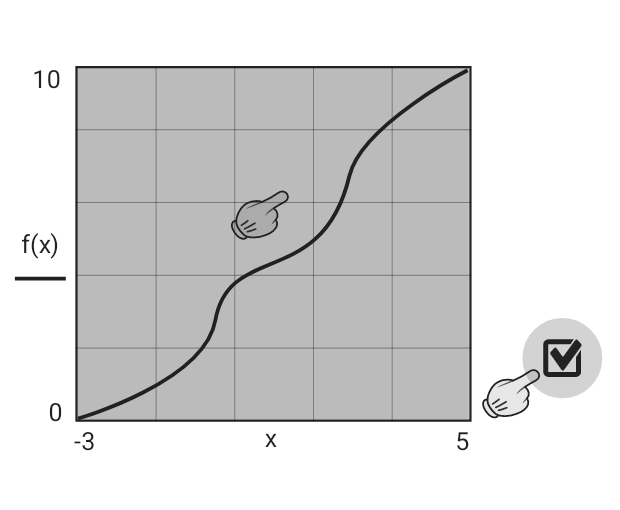
\includegraphics[width=0.45\textwidth]{graphics/function_plot_fig5.png} \end{tabular}\end{center}

При нажатии на эту кнопку откроется
окно настроек графика, где можно
изменить как размер, так и стиль
области графика. К примеру, мы
можем уменьшить высоту и включить
координатные оси вместо рамки:
\begin{center}\begin{tabular}{c} 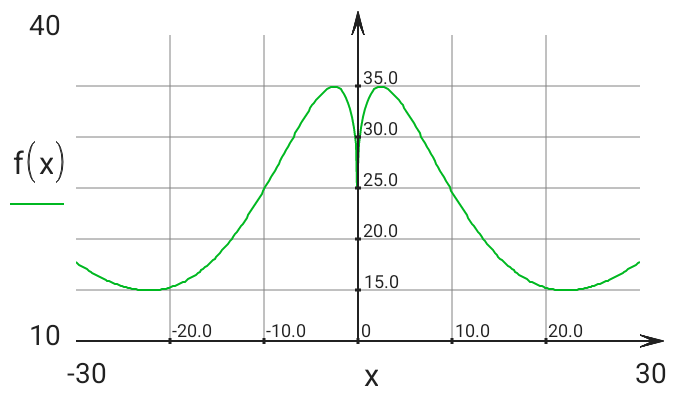
\includegraphics[width=0.45\textwidth]{graphics/function_plot_fig6.png} \end{tabular}\end{center}

Толщину, цвет и стиль линий
графика, а также маркеры значений
функции можно изменить в окне
''Настройка линии''. Это окно
вызывается долгим нажатием на
линию-маркер, расположенную под
выражением функции слева от поля
графика:
\begin{center}\begin{tabular}{c} 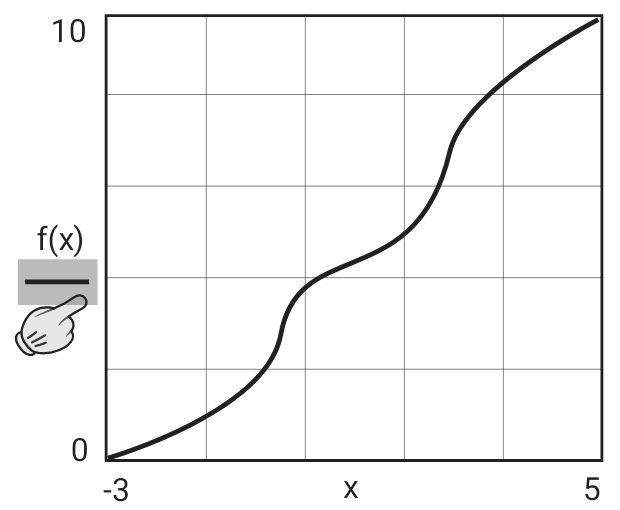
\includegraphics[width=0.45\textwidth]{graphics/function_plot_fig7.png} \end{tabular}\end{center}

Например, построим пунктирный
график:
\begin{center}\begin{tabular}{c} 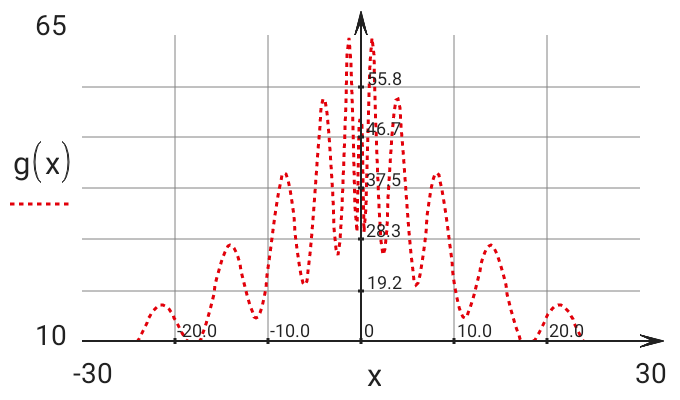
\includegraphics[width=0.45\textwidth]{graphics/function_plot_fig8.png} \end{tabular}\end{center}

Масштаб осей (линейный или
логарифмический),  количество
линий сетки по горизонтали и
вертикали, а также цвет линий
сетки можно изменить в окне
''Настройка сетки''. Это окно
вызывается долгим нажатием в
пустые области снизу от графика,
между минимальным значением и
выражением для аргумента, а также
между аргументом и его
максимальным значением:
\begin{center}\begin{tabular}{c} 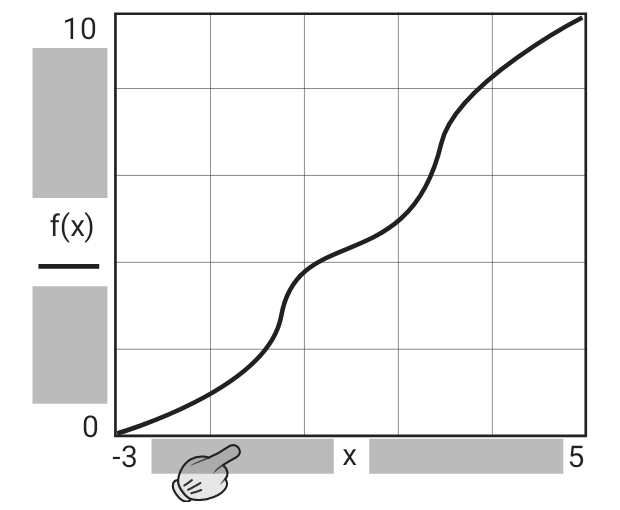
\includegraphics[width=0.45\textwidth]{graphics/function_plot_fig9.png} \end{tabular}\end{center}
\begin{center}\begin{tabular}{c} 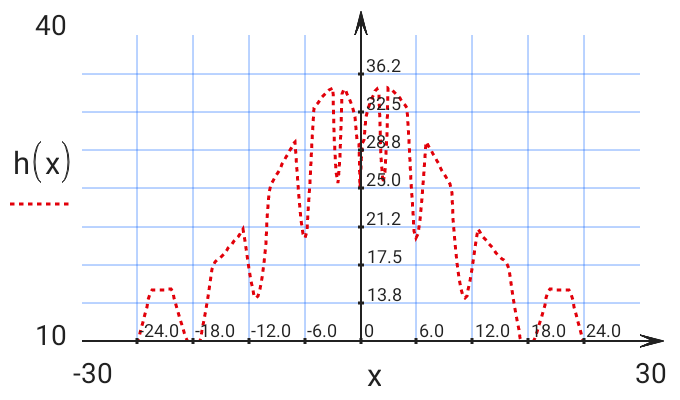
\includegraphics[width=0.45\textwidth]{graphics/function_plot_fig10.png} \end{tabular}\end{center}

Чтобы полностью отключить сетку,
необходимо задать нулевое
количество линий по горизонтали и
вертикали.

\section{Пример: полярный график}
% This is auto-generated file: do not edit!
% Exported from microMathematics Plus, version 2.23.2


Сейчас мы построим несколько
графиков функций в полярной
системе координат. Каждая точка в
этой системе определяется
расстоянием r от начала координат
и углом f относительно оси
абсцисс.
\begin{center}\begin{tabular}{c} 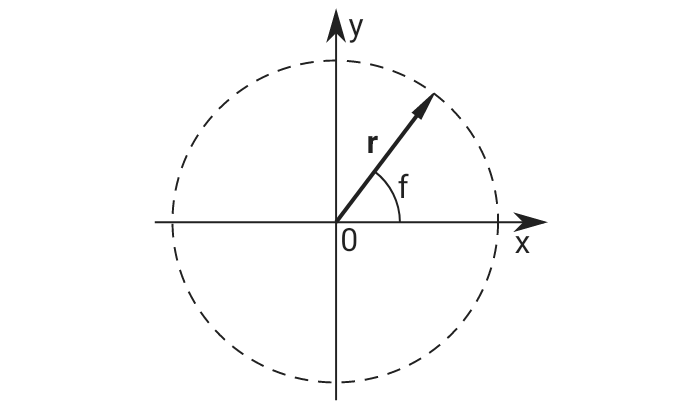
\includegraphics[width=0.45\textwidth]{graphics/polar_plot_fig1.png} \end{tabular}\end{center}

Угловая координата f будет являться
нашей независимой переменной,
которую мы зададим в виде
интервала:
\begin{center}\begin{tabular}{c}
  $f := \left[ 0.01,\, 0.05 \,..\, 300 \right]$
\end{tabular}\end{center}

Расстояние от начала координат r -
это зависимая переменная. Каждую
пару значений f и r можно
пересчитать в декартовы координаты
x и y, используя следующие
формулы:
\begin{center}\begin{tabular}{cc}
  $x(r) := r \cdot cos \left( f\right) $ &
  $y(r) := r \cdot sin \left( f\right) $ \cr
\end{tabular}\end{center}

\subsection{Улитка}

Первую функцию будем определять в
три шага. На первом шаге введём
функцию, которая описывает простое
''колесо''. Эта функция зависит от
трёх коэффициентов A, B, q. Их
изменение позволяет значительно
менять вид получаемых кривых: 
\begin{center}\begin{tabular}{ccc}
  $A := 1.1$ &
  $B := 1.271$ &
  $q := 2$ \cr
\end{tabular}\end{center}
\begin{center}\begin{tabular}{c}
  $r1(f) := A + 2 \cdot {sin \left( B \cdot f\right) }^{q}$
\end{tabular}\end{center}

Далее добавим поле графика,
используя кнопку ''Вставить'' на
верхней панели действий или
кнопку ''Вставить график функции''
на нижней панели:
\begin{center}\begin{tabular}{c} 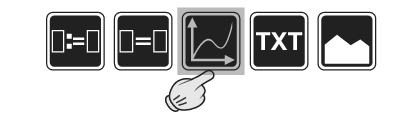
\includegraphics[width=0.45\textwidth]{graphics/polar_plot_fig2.png} \end{tabular}\end{center}

Однако вместо пары f и r мы должны
использовать в поле графика их
декартовы образы, которые
получаются, если взять приведённые
выше формулы преобразований и
подставить в них r1(f) в качестве
символьного аргумента:
\begin{center}\begin{tabular}{c} 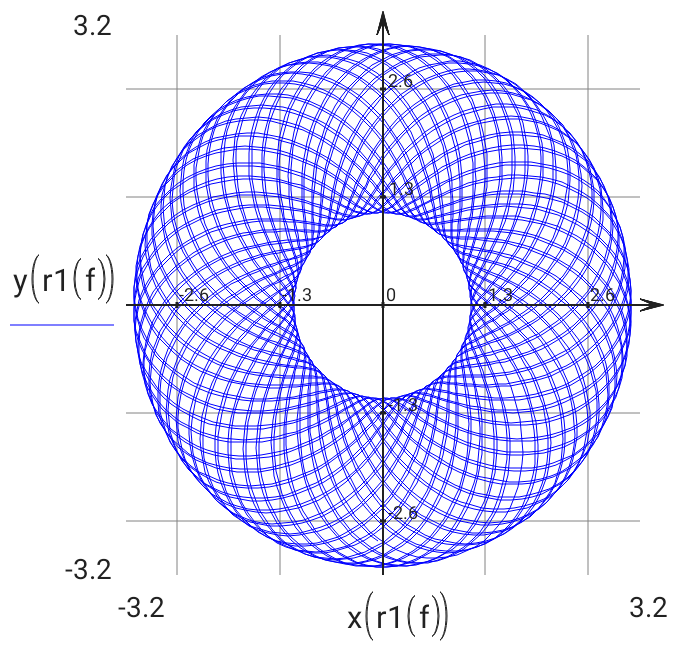
\includegraphics[width=0.45\textwidth]{graphics/polar_plot_fig3.png} \end{tabular}\end{center}

Затем немного модифицируем наше
''колесо'':
\begin{center}\begin{tabular}{c}
  $r2(f) := A + 2 \cdot {sin \left( B \cdot f + 1 \cdot r1 \left( f\right) \right) }^{q}$
\end{tabular}\end{center}
\begin{center}\begin{tabular}{c} 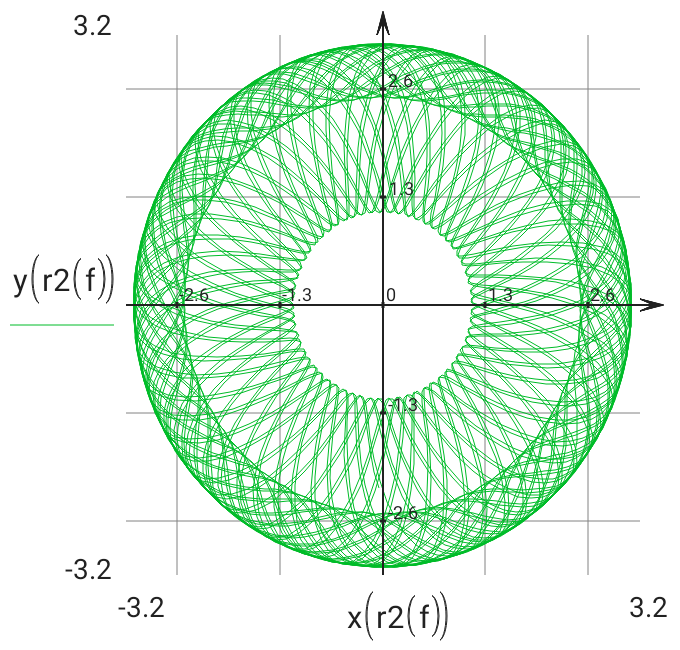
\includegraphics[width=0.45\textwidth]{graphics/polar_plot_fig4.png} \end{tabular}\end{center}

Наконец, зададим итоговую функцию
скалированием функции r2(f),
используя при этом операцию
преобразования вещественного числа
в целое, которая выглядит как
ступенчатая функция. В итоге,
получилась вот такая замечательная
улитка:
\begin{center}\begin{tabular}{c}
  $r(f) := r2 \left( f\right)  \cdot floor \left( f\right)  / 10$
\end{tabular}\end{center}
\begin{center}\begin{tabular}{c} 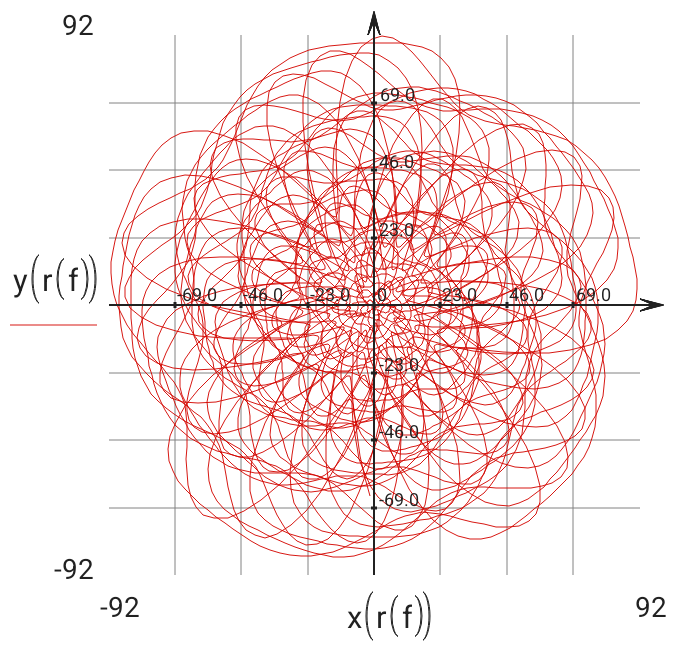
\includegraphics[width=0.45\textwidth]{graphics/polar_plot_fig5.png} \end{tabular}\end{center}

\subsection{Японский клён}

Японский клён получил широкую
известность благодаря необычным
формам и окраске своих листьев.
Данный пример показывает, как
такой лист может быть описан
математически и нарисован как
кривая в полярной системе
координат:
\begin{center}\begin{tabular}{c}
  $f := \left[ 0.01,\, 0.02 \,..\, 100 \right]$
\end{tabular}\end{center}
\begin{center}\begin{tabular}{cc}
  $x(r) := r \cdot cos \left( f\right) $ &
  $y(r) := r \cdot sin \left( f\right) $ \cr
\end{tabular}\end{center}
\begin{center}\begin{tabular}{c}
  $s1(f) := \left( 1 + sin \left( f\right)  \right) \cdot \left( 1 - 0.9 \cdot  \left| sin \left( 4 \cdot f\right)  \right|  \right)$
\end{tabular}\end{center}
\begin{center}\begin{tabular}{c}
  $s2(f) := 0.9 + 0.05 \cdot cos \left( 200 \cdot f\right) $
\end{tabular}\end{center}
\begin{center}\begin{tabular}{c}
  $r(f) := floor \left( f\right)  \cdot s1 \left( f\right)  \cdot s2 \left( f\right)  + random \left( 2\right)  - 1$
\end{tabular}\end{center}
\begin{center}\begin{tabular}{c} 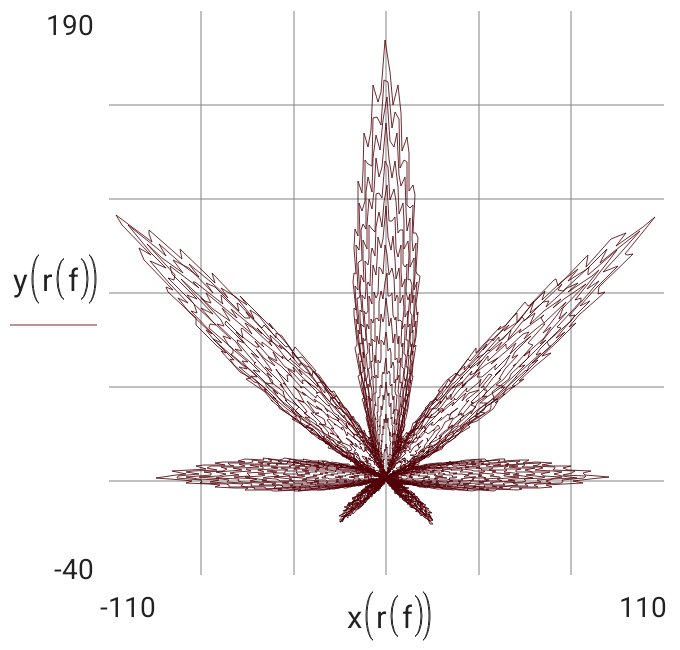
\includegraphics[width=0.45\textwidth]{graphics/polar_plot_fig6.png} \end{tabular}\end{center}

http://en.wikipedia.org/wiki/Acer\_palmatum

\section{Пример: 3D график}
% This is auto-generated file: do not edit!
% Exported from microMathematics Plus, version 2.23.0


Данный пример демонстрирует
построение трёхмерных графиков
для трёх различных функций двух
переменных.

Для начала, определим интервалы
изменения двух независимых
переменных x и y. Область
изменения переменной x зависит от
количества точек по оси абсцисс N,
а также от минимального и
максимального значений x1 и x2:
\begin{center}\begin{tabular}{ccc}
  $N := 300$ &
  $x1 := -2$ &
  $x2 := 2$ \cr
\end{tabular}\end{center}
\begin{center}\begin{tabular}{c}
  $x := \left[ x1,\, x1 +  \left| x2 - x1 \right|  / N \,..\, x2 \right]$
\end{tabular}\end{center}

Область изменения переменной y по
оси ординат определим аналогично:
\begin{center}\begin{tabular}{ccc}
  $M := 300$ &
  $y1 := -3$ &
  $y2 := 3$ \cr
\end{tabular}\end{center}
\begin{center}\begin{tabular}{c}
  $y := \left[ y1,\, y1 +  \left| y2 - y1 \right|  / M \,..\, y2 \right]$
\end{tabular}\end{center}

Первая функция является
произведением синуса и косинуса
степенных функций:
\begin{center}\begin{tabular}{c}
  $F(x,y) := sin \left( 3 \cdot {x}^{2}\right)  \cdot cos \left( {y}^{2}\right) $
\end{tabular}\end{center}

Для создания контурного графика
используйте кнопку ''Вставить'' на
верхней панели инструментов или
кнопку ''Вставить 3D график'' на
нижней панели:
\begin{center}\begin{tabular}{c} 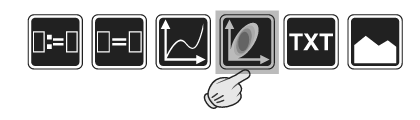
\includegraphics[width=0.45\textwidth]{graphics/three_d_plot_fig1.png} \end{tabular}\end{center}

В центральное поле внизу графика
вводится или имя функции с двумя
аргументами, или выражение,
которое явно зависит от двух
переменных интервального типа:
\begin{center}\begin{tabular}{c} 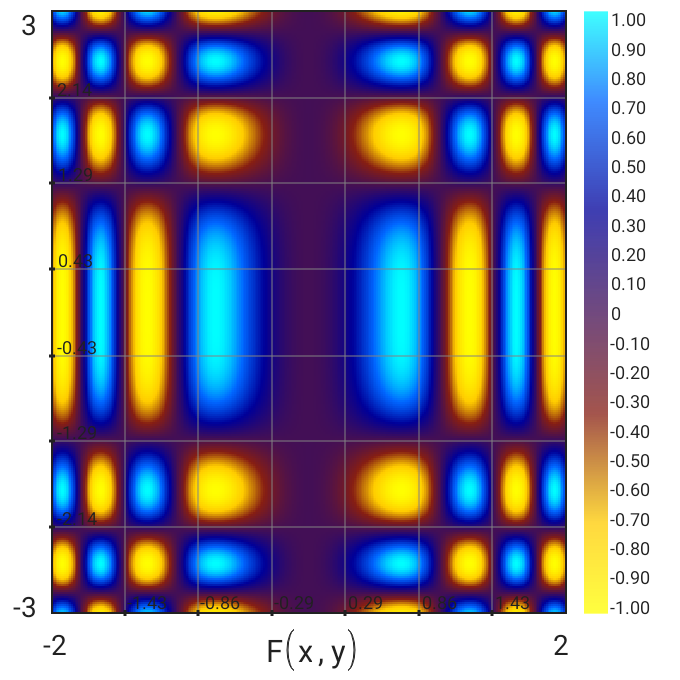
\includegraphics[width=0.45\textwidth]{graphics/three_d_plot_fig2.png} \end{tabular}\end{center}

Также же как и для графика функции
одной переменной, размер и стиль
трёхмерного графика изменяется в
окне настроек графика (см. пример
''График функции'' из навигатора
приложения). Это окно можно
вызвать кнопкой ''Настройки
объекта'', которая появляется при
долгом нажатием на центральную
область графика.

Дополнительно можно изменить
цветовую палитру и количество
маркеров по оси z. Это делается в
диалоговом окне ''Цветовая схема'',
которое вызывается долгим нажатием
на цветовую панель справа от
области графика.
\begin{center}\begin{tabular}{c}
  $R(x,y) := sin \left( 5 \cdot {x}^{2} \cdot \left( y - x \right)\right) $
\end{tabular}\end{center}
\begin{center}\begin{tabular}{c} 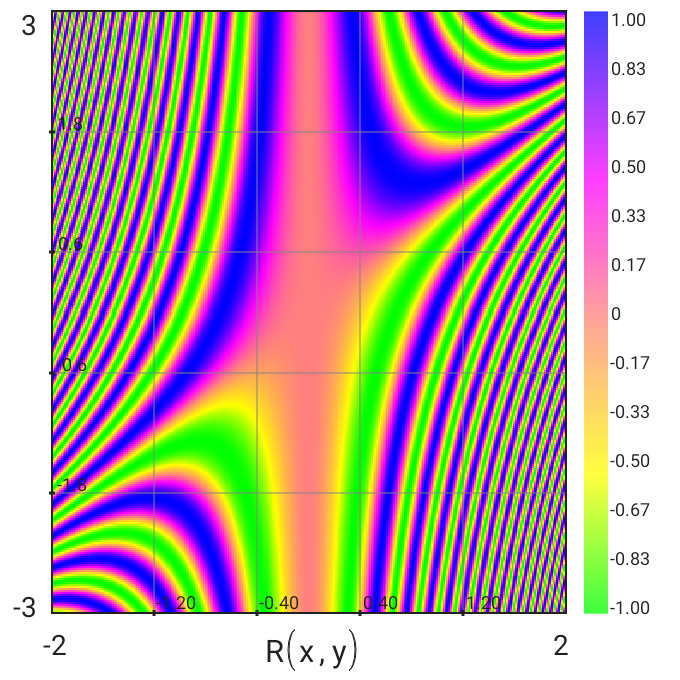
\includegraphics[width=0.45\textwidth]{graphics/three_d_plot_fig3.png} \end{tabular}\end{center}

Функцию двух переменных также можно
отобразить и в виде поверхности.
Этот режим отображения включается
в окне настроек графика. Как уже
говорилось, оно вызывается
нажатием на плавающую кнопку
''Настройки объекта'' после долгого
нажатия на поле графика. Для
примера, построим такую
поверхность, используя промежуточные
массивы для ускорения вычислений:
\begin{center}\begin{tabular}{cccc}
  $N := 100$ &
  $n := \left[ 0,\, 1 \,..\, N \right]$ &
  $x1 := -15$ &
  $x2 := 15$ \cr
\end{tabular}\end{center}
\begin{center}\begin{tabular}{cccc}
  $M := 100$ &
  $m := \left[ 0,\, 1 \,..\, M \right]$ &
  $y1 := -15$ &
  $y2 := 15$ \cr
\end{tabular}\end{center}
\begin{center}\begin{tabular}{c}
  $x_{n}  := {\left( x1 +  \left( x2 - x1\right)  \cdot n / N \right)}^{2}$
\end{tabular}\end{center}
\begin{center}\begin{tabular}{c}
  $y_{m}  := {\left( y1 +  \left( y2 - y1\right)  \cdot m / M \right)}^{2}$
\end{tabular}\end{center}
\begin{center}\begin{tabular}{c}
  $r_{n,\, m}  := 0.04 \cdot x_{n}  + 0.02 \cdot y_{m} $
\end{tabular}\end{center}
\begin{center}\begin{tabular}{c}
  $t_{n,\, m}  := \left( x_{n}  + 0.05 \cdot y_{m}  \right) \cdot exp \left( 1 - r_{n,\, m} \right) $
\end{tabular}\end{center}
\begin{center}\begin{tabular}{c}
  $F_{n,\, m}  := \frac{sin \left( x_{n}  + 0.1 \cdot y_{m} \right) }{0.15 + r_{n,\, m} } + \frac{t_{n,\, m} }{10}$
\end{tabular}\end{center}
\begin{center}\begin{tabular}{c} 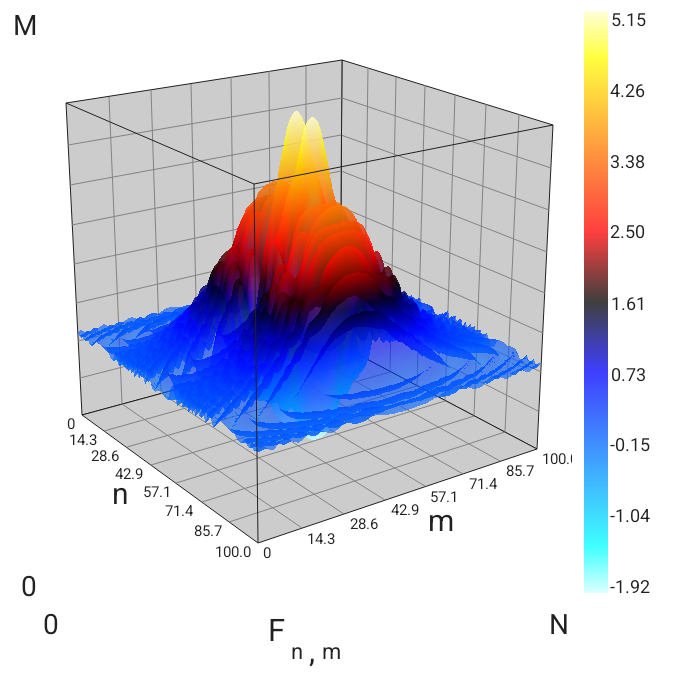
\includegraphics[width=0.45\textwidth]{graphics/three_d_plot_fig4.png} \end{tabular}\end{center}

Если функция отображается в виде
поверхности, то в окне ''Настройка
графика'' можно настроить для неё
дополнительные параметры: показ
линий сетки, режим закрашивания,
прозрачность, углы поворота и
наклона поверхности. Например,
посмотрим на предыдущую 
поверхность под другим углом:
\begin{center}\begin{tabular}{c} 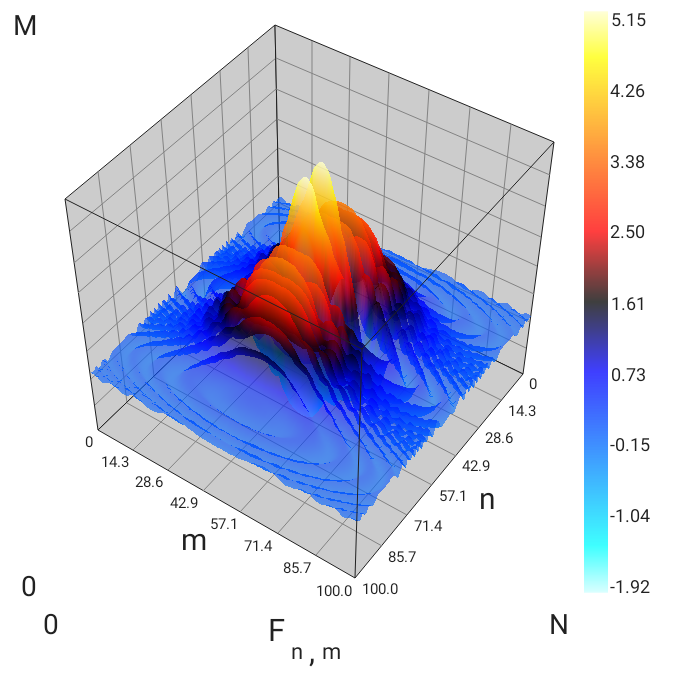
\includegraphics[width=0.45\textwidth]{graphics/three_d_plot_fig5.png} \end{tabular}\end{center}

\section{Пример: ряды и интегралы}
% This is auto-generated file: do not edit!
% Exported from microMathematics Plus, version 2.23.0


Данный пример демонстрирует
вычисление степенных рядов и
интегралов.

\subsection{Ряд Тейлора}

Рядом Тейлора является разложение
функции в бесконечный степенной
ряд, коэффициенты которого
вычисляются с использованием
производных исходной функции.

Например, разложение в ряд Тейлора
функции в окрестности точки x, где
количество членов степенного ряда
равно N, обозначим как Ts(x,N):
\begin{center}\begin{tabular}{c}
  $Ts(x,N) := \displaystyle\sum_{n=0}^{N} \frac{{ \left( -1\right) }^{n}}{\left( 2 \cdot n \right)! } \cdot {x}^{2 \cdot n}$
\end{tabular}\end{center}

Данное разложение аппроксимирует
функцию косинуса:
\begin{center}\begin{tabular}{c}
  $s(x) := cos \left( x\right) $
\end{tabular}\end{center}

Построим график обеих функций для
одного и того же интервала. На
первый взгляд, обе кривые
идентичны:
\begin{center}\begin{tabular}{c}
  $x := \left[ 0,\, 0.1 \,..\, 2 \cdot {\pi} \right]$
\end{tabular}\end{center}
\begin{center}\begin{tabular}{c} 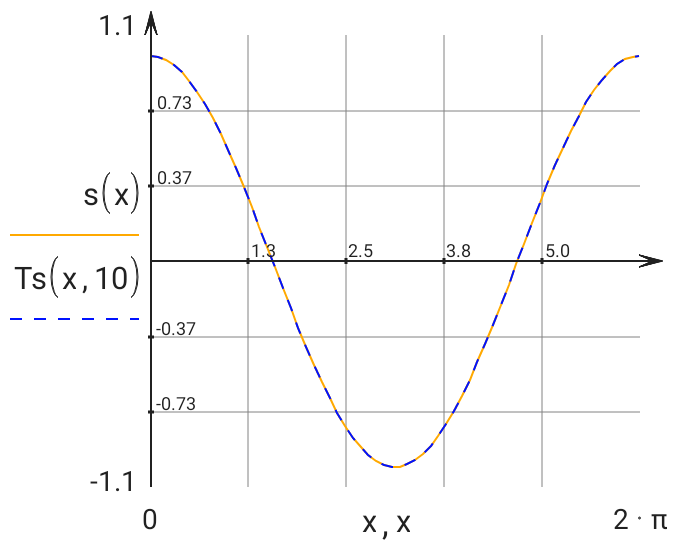
\includegraphics[width=0.45\textwidth]{graphics/series_and_integrals_fig1.png} \end{tabular}\end{center}

На самом же деле, сумма ряда
Ts(x,N) вычислена с погрешностью,
которая обусловлена конечным
количеством членов ряда N. Введём
функцию невязки $\Delta$(x,N), которая
описывает эту погрешность:
\begin{center}\begin{tabular}{c}
  ${\Delta}(x,N) :=  \left| s \left( x\right)  - Ts \left( x,\, N\right)  \right| $
\end{tabular}\end{center}

Построим график этой функции в
зависимости от количества членов
ряда. В данном случае, удобнее
использовать логарифмическую ось
ординат, которая включается в окне
''Настройка сетки'' графика. Тогда
мы увидим, что порядок погрешности
линейно уменьшается с увеличением
количества членов ряда:
\begin{center}\begin{tabular}{c}
  $N := \left[ 3,\, 4 \,..\, 13 \right]$
\end{tabular}\end{center}
\begin{center}\begin{tabular}{c} 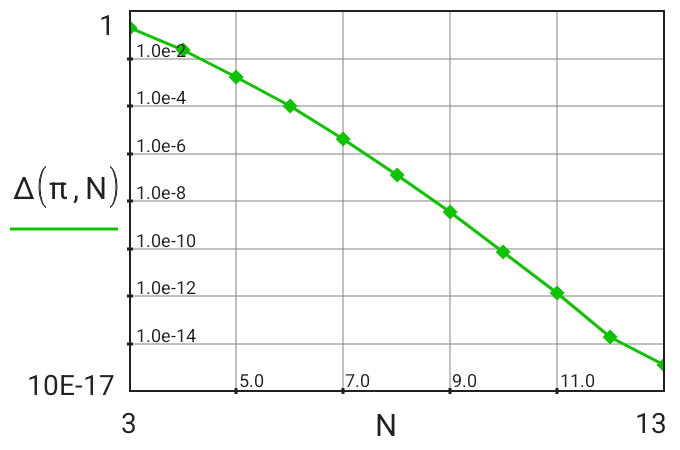
\includegraphics[width=0.45\textwidth]{graphics/series_and_integrals_fig2.png} \end{tabular}\end{center}

\subsection{Биномиальный ряд}

Рассмотрим степенную функцию
\begin{center}\begin{tabular}{c}
  $f(x,{\alpha}) := {\left( 1 + x \right)}^{{\alpha}}$
\end{tabular}\end{center}

Эту функцию можно разложить в
биномиальный ряд:
\begin{center}\begin{tabular}{c}
  $Tf(x,{\alpha},N) := \displaystyle\sum_{n=0}^{N}  \left( \displaystyle\prod_{k=1}^{n} \frac{{\alpha} - k + 1}{k}\right)  \cdot {x}^{n}$
\end{tabular}\end{center}

Также как и в предыдущем примере,
можно построить графики обеих
функций. Несмотря на то, что
исходная и аппроксимированная
функции визуально совпадают, здесь
также имеется погрешность,
связанная с конечным числом членов
ряда:
\begin{center}\begin{tabular}{c} 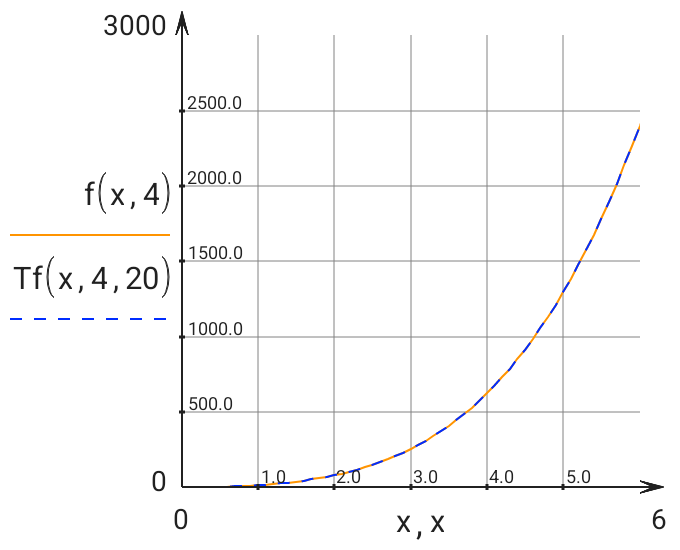
\includegraphics[width=0.45\textwidth]{graphics/series_and_integrals_fig3.png} \end{tabular}\end{center}

\subsection{Интегралы}

Программа также предоставляет
возможность вычисления
определённых интегралов методом
Симпсона. К примеру, можно
вычислять интегралы с
использованием элемента ''Текстовый
результат'':
\begin{center}\begin{tabular}{c}
  $\displaystyle\int_{0}^{3 \cdot pi / 2}{cos \left( \frac{2 \cdot x}{9}\right) }^{-2}\, dx = 7.79423$
\end{tabular}\end{center}

Аналитическое решение для данного
интеграла выглядит следующим
образом:
\begin{center}\begin{tabular}{ccc}
  $I := \frac{9 \cdot \sqrt{3} }{2}$ &
  ,    &
  $I = 7.79423$ \cr
\end{tabular}\end{center}

Так как интеграл найден не
аналитически, а с использованием
численного метода, то имеет место
быть следующая погрешность:
\begin{center}\begin{tabular}{c}
  $\displaystyle\int_{0}^{3 \cdot pi / 2}{cos \left( \frac{2 \cdot x}{9}\right) }^{-2}\, dx - I = 4.26681E-9$
\end{tabular}\end{center}

Эта погрешность зависит от
параметра ''Значимые цифры в
результате''. Данный параметр
задаётся в окне ''Свойства
документа'', которое вызывается из
верхней панели действий:
\begin{center}\begin{tabular}{c} 
\includegraphics[width=0.45\textwidth]{graphics/series_and_integrals_fig4.png} \end{tabular}\end{center}

При увеличении этого параметра,
точность вычисления интеграла
увеличивается, но увеличивается
также и время, необходимое для его
вычисления.

\section{О программе}

% This is the second part of the file about_micromath_ru.tex
\subsection{Авторы}

\begin{enumerate}
\item Михаил Кулеш,
mikhail.kulesh@gmail.com

\item Caio Roberto Ramos da Silva
(перевод на португальский),
caiorrs@gmail.com

\item Yubin Hsu
(перевод на китайский),
yubin.taiwan@gmail.com

\item Linsui
(перевод на китайский),
linsui555@gmail.com

\item Diego Sanguinetti
(перевод на испанский)
\end{enumerate}

\subsection{Иконка}

Иконка приложения получена в нём же
с использованием функции,
определённой в полярной системе
координат:
\begin{center}\begin{tabular}{c}
  $f := \left[ 0.01,\, 0.03 \,..\, 150 \right]$
\end{tabular}\end{center}
\begin{center}\begin{tabular}{c}
  $s(f) := 4 + sin \left( 5 \cdot f\right)  + \frac{sin \left( 10 \cdot f\right) }{2} + \frac{sin \left( 60 \cdot f\right) }{6}$
\end{tabular}\end{center}
\begin{center}\begin{tabular}{c}
  $r(f) := 0.9 \cdot \left( 1 + f / 50 \right) \cdot s \left( f\right) $
\end{tabular}\end{center}
\begin{center}\begin{tabular}{c}
  $x(f) := r \left( f\right)  \cdot cos \left( f\right) $
\end{tabular}\end{center}
\begin{center}\begin{tabular}{c}
  $y(f) := r \left( f\right)  \cdot sin \left( f\right) $
\end{tabular}\end{center}
\begin{center}\begin{tabular}{c} 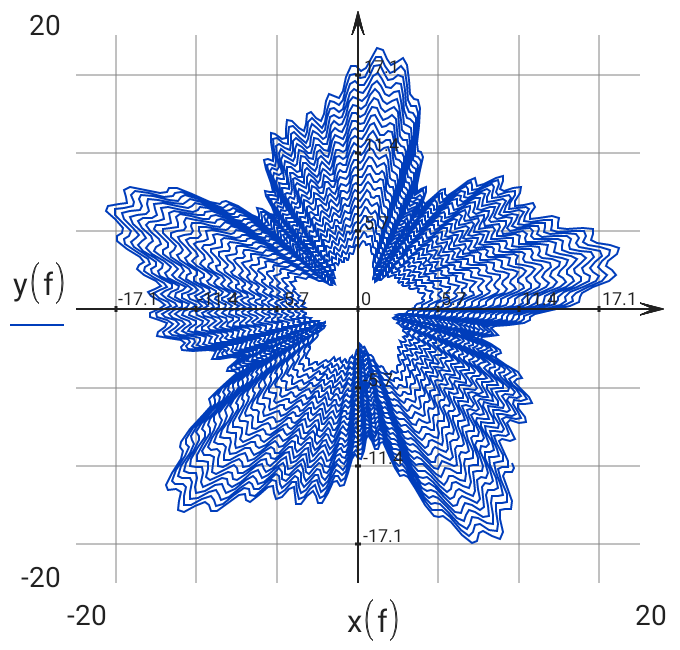
\includegraphics[width=0.45\textwidth]{graphics/about_micromath_fig1.png} \end{tabular}\end{center}

\subsection{Лицензия}

Copyright © 2014-2022 by Mikhail Kulesh
под лицензией GNU General Public License,
Version 3:
www.gnu.org/licenses/gpl-3.0

\end{document}
